\chaptertoc{}

\vspace{1em}

At redshifts between 0 and 2, galaxies can be used as tracers of
the matter distribution. With the statistics of the galaxy distribution 
we can measure characteristic scale of the baryon acoustic oscillations (BAO), 
as well as extract information about the growth-rate of structures from 
the anisotropies caused by redshift-space distortions (RSD). 
As presented in Chapter~\ref{chap:intro}, BAO and RSD are powerful 
probes of dark-energy and theories of gravity. 

In this Chapter, I overview my contributions for the study of dark-energy 
with galaxy clustering. Section~\ref{galaxies:catalogue} describes how to 
create a galaxy clustering catalogue from the spectroscopic observations, 
including and correcting for most observational systematic effects.
In section~\ref{galaxies:bao} I present the BAO measurements I performed 
with the SDSS sample of luminous red galaxies, while section~\ref{galaxies:rsd}
focus on the RSD constraints. Section~\ref{galaxies:joint} 
overviews recent work carried out by my PhD students Tyann Dumerchat 
and Vincenzo Aronica on the joint analysis of galaxy clustering in 
Fourier and configuration space. 

The work described in this chapter is published in the following 
articles: 
\cite{bautistaSDSSIVExtendedBaryon2018, 
bautistaCompletedSDSSIVExtended2020,
gil-marinCompletedSDSSIVExtended2020,
rossCompletedSDSSIVExtended2020,
zhaoCompletedSDSSIVExtended2021,
%dumerchatJoint2022
}. 

\section{From redshifts to clustering catalogues}
\label{galaxies:catalogue}

An essential step in the cosmological analysis of galaxy survey data is 
to convert convert a list of galaxy redshifts (see Chapter~\ref{chap:spectro}) 
into a catalogue from which we can define overdensities 
$\delta_n(\vec{x}) = n(\vec{x})/\bar{n} - 1$, where $n(\vec{x})$ is the 
number density 
of galaxies in a volume element located at position $\vec{x}$. 
The quantity $\bar{n}$ is the average galaxy number density over the probed 
\emph{volume}. Therefore, it is important to 1) define precisely what is the 
volume observed, or in jargon terms, the survey window function; and 
2) to make sure that the number density of galaxies is tracing the actual 
cosmological fluctuations and not any spurious contamination. 

The simplest form of survey window function would be some function of position $\vec{x}$ 
that is 1 if the volume was ``observed'' and 0 else. 
One way to define this function is using a Poisson random sampling 
of the volume with points, with some arbitrary higher number density than the 
galaxy average number density (typically between 20 or 50 times higher). 
The list of points is referred to as the \emph{random} catalogue. 
In practice, the random catalogue is more complicated and accounts for 
observational completeness and systematic effects, as described below. 

In SDSS analyses, the random catalogue is a combination of an angular footprint 
and a radial distribution, both trying to matching the galaxy sample as better as possible. 

I describe now the procedure to define the angular footprint. 
The starting footprint is the same where the target selection 
(section~\ref{spectro:target})
was previously defined. 
Figure~\ref{fig:eboss_footprint} displays the eBOSS footprint for the three tracers 
(LRGs, ELGs and QSOs) compared to the BOSS footprint and the stellar density map from Gaia. 
Regions with bad photometric or around 
bright stars are masked out by removing randoms belonging to these regions
(or assigning them a null weight). 
After tiling, fibre assignement and spectroscopic observations, the footprint 
can be divided into an unique set of sectors. Each sector corresponds to regions
observed by one or more plates. The \emph{fibre completeness} of each sector is 
defined as the ratio between the number of spectroscopically observed targets and 
the number of available targets in the sector. Random points are sub-sampled or de-weighted 
following the fibre completeness to account for it. 

\begin{figure}
    \centering 
    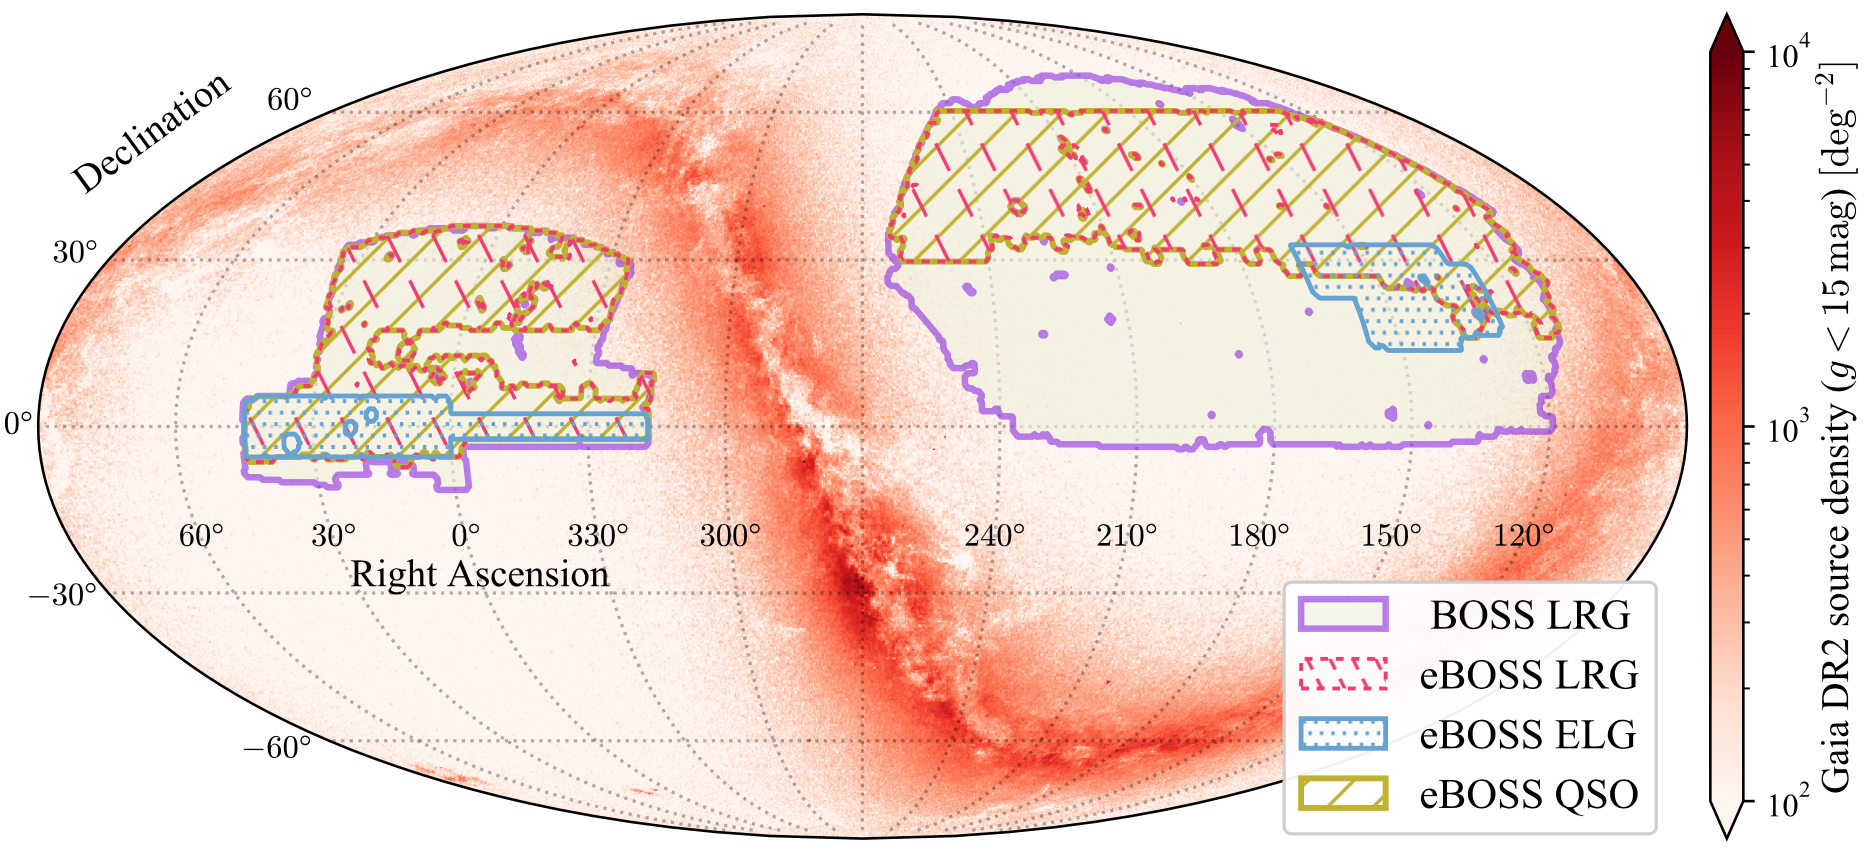
\includegraphics[width=0.9\textwidth]{fig/galaxies/eboss_footprint.png}
    \caption{ The DR16 footprint for each eBOSS tracer: Luminous Red Galaxies (LRG), 
    Emission Line Galaxies (ELG) and quasars (QSO). The BOSS DR12 LRGs area is also shown, 
    as well as the density map of Gaia DR2 sources with $g < 15$ mag.
    Figure extracted from \cite{zhaoCompletedSDSSIVExtended2021}.} 
    \label{fig:eboss_footprint}
\end{figure}

Some targets cannot be observed due to 
its proximity to another observed target and the finite size of fibres, corresponding 
to 62 arcseconds in the sky. We refer to these events as \emph{fibre collisions}. 
Collisions might happen not only to pairs of galaxies, but to any group of targets with 
linking lengths smaller than 62 arcsec. Depending on the number of plates observing 
a giving sector, some collisions might be solved but the missing ones might 
impact the measured clustering on small scales if not corrected. 
While there are several methods to solve collisions 
(\cite{guoNewMethodCorrect2012, bianchiUnbiasedClusteringEstimation2017}),
we used the simplest up-weighting technique, where the nearest observed galaxy 
is up-weighted by the number of non-observed targets within the collision group. 
This assumes that non-observed targets are also galaxies of the same target type and 
that they are physically close (angularly and radially) to the observed ones.
On scales above a few \hmpc, this simple correction is a good approximation. 

Two additional sets of weights are defined to correct for spurious density 
fluctuations which contaminate the cosmological fluctuations. 
These weights are applied to the galaxies themselves. 

The first set of weights corrects for angular fluctuations caused 
by correlations between galaxy number density and photometry-related quantities,
such as Galactic extinction, stellar density, imaging depth or sky flux.
They are commonly referred to as \emph{photometric weights}. 
Figure~\ref{fig:photo_systematics_lrg} displays these correlations 
for the LRG sample both before and after corrections. 
For the analysis of eBOSS DR16 LRGs, I have 
implemented\footnote{\url{https://github.com/julianbautista/eboss_clustering/blob/master/python/systematic_fitter.py}} 
a multi-dimension 
linear regression that assumes these correlations are linear and 
accounts for the fact that some photometric quantities are correlated between themselves 
(e.g., stellar density and Galactic extinction).
This multi-linear method is based on work described in \cite{prakashSDSSIVExtendedBaryon2016}.
Of course, more advanced methods have been developed since then, based on 
machine learning algorithms 
(\cite{rezaieImprovingGalaxyClustering2020, chaussidonAngularClusteringProperties2021}).
It is important to evaluate the performance of these algorithms with mock catalogues
where we add artificial contamination 
and quantify how well we recover the initial raw power spectrum after correcting for them. 
There is a risk of overfitting and removing some large-scale cosmological modes which 
can be harmful for clustering analysis, particularly those aiming at measuring 
primordial non-Gaussianity 
(\cite{rezaiePrimordialNonGaussianityCompleted2021, muellerClusteringGalaxiesCompleted2021}).

\begin{figure}
    \centering 
    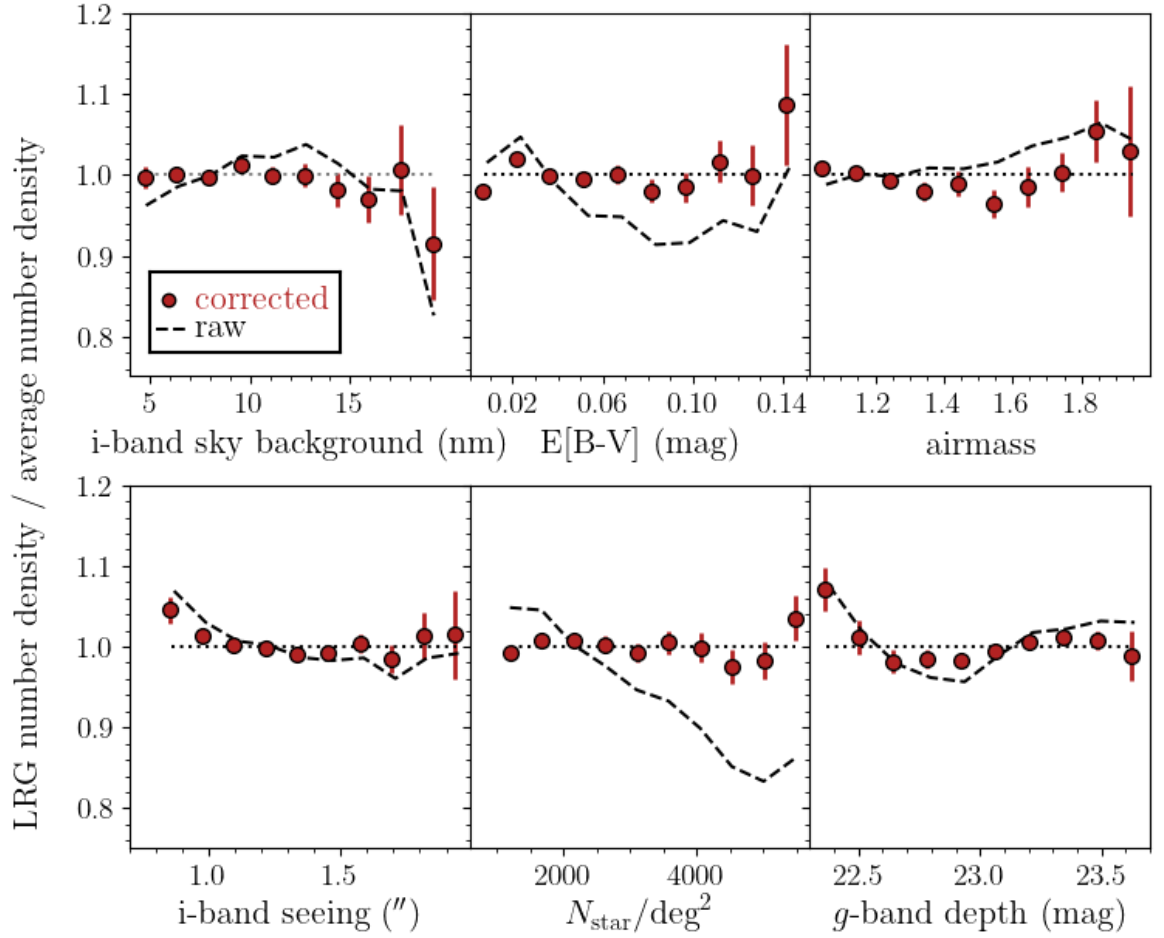
\includegraphics[width=0.7\textwidth]{fig/galaxies/photometric_weights_lrg.png}
    \caption{ Fluctuations in the angular LRG density as a function of 
    various imaging properties and Galactic foregrounds. 
    The dashed curves show these fluctuations before any correction 
    while red points show the result of applying a linear correction for 
    stellar density and Galactic extinction. 
    Figure extracted from \cite{rossCompletedSDSSIVExtended2020}.} 
    \label{fig:photo_systematics_lrg}
\end{figure}

A second set of weights corrects for the fact for the so-called \emph{redshift failures}, 
i.e., the fact that some spectra with low signal-to-noise ratio (S/N)
do not yield a statistically significant redshift measurement. 
If they were randomly distributed across the sky, failures would not be an issue for 
clustering. However, given the instrument configuration and throughput, these failures 
imprint a pattern in the sky which contaminates clustering. 
In the left panel of Figure~\ref{fig:eboss_zfailures} we see the average failure rate 
of eBOSS LRGs as a function of position in the focal plane. The reason for this pattern
is that the fibres at the side edges of the focal plane transport light to the edges 
of the camera CCDs and therefore have a lower-than-average throughput, or lower signal-to-noise
ratio. 
The right panel of Figure~\ref{fig:eboss_zfailures} shows the 
dependency of the average redshift failure rate as a function of the signal-to-noise
ratio of the observation\footnote{The signal-to-noise ratio of an observation is 
a function of the signal-to-noise ratio of all observed spectra and their magnitudes.}, 
which is the actual underlying reason for the failure rates. 
When modelling these dependencies of failure rates with S/N (or fibre number or focal plane
position), one can correct these spurious fluctuations by assigning a weight 
inversely proportional to the modelled rate. 
These are the so called \emph{redshift-failure weights} and are assigned to the 
galaxies with confident redshift measurements, to compensate for the eventual 
non-confident ones at the same location in the focal plane. 

\begin{figure}
    \centering 
    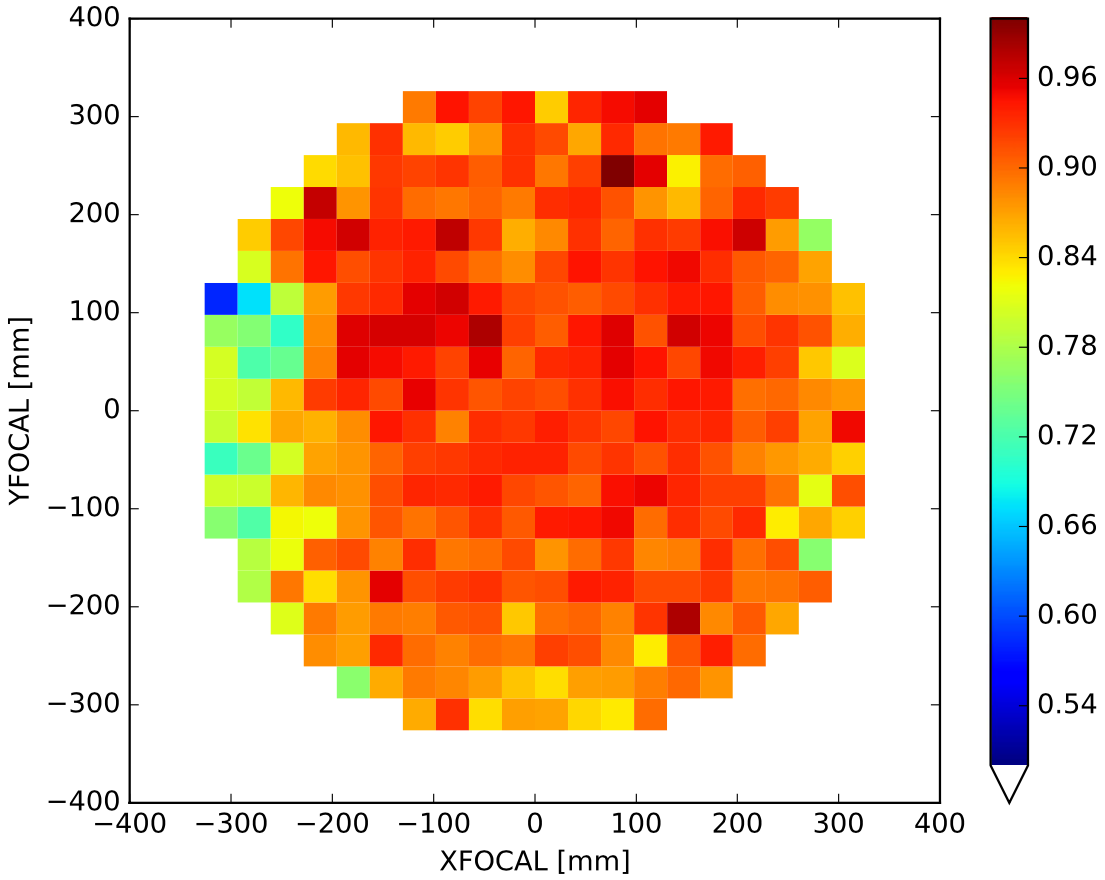
\includegraphics[width=0.49\textwidth]{fig/galaxies/eboss_z_failures_focalplane.png}
    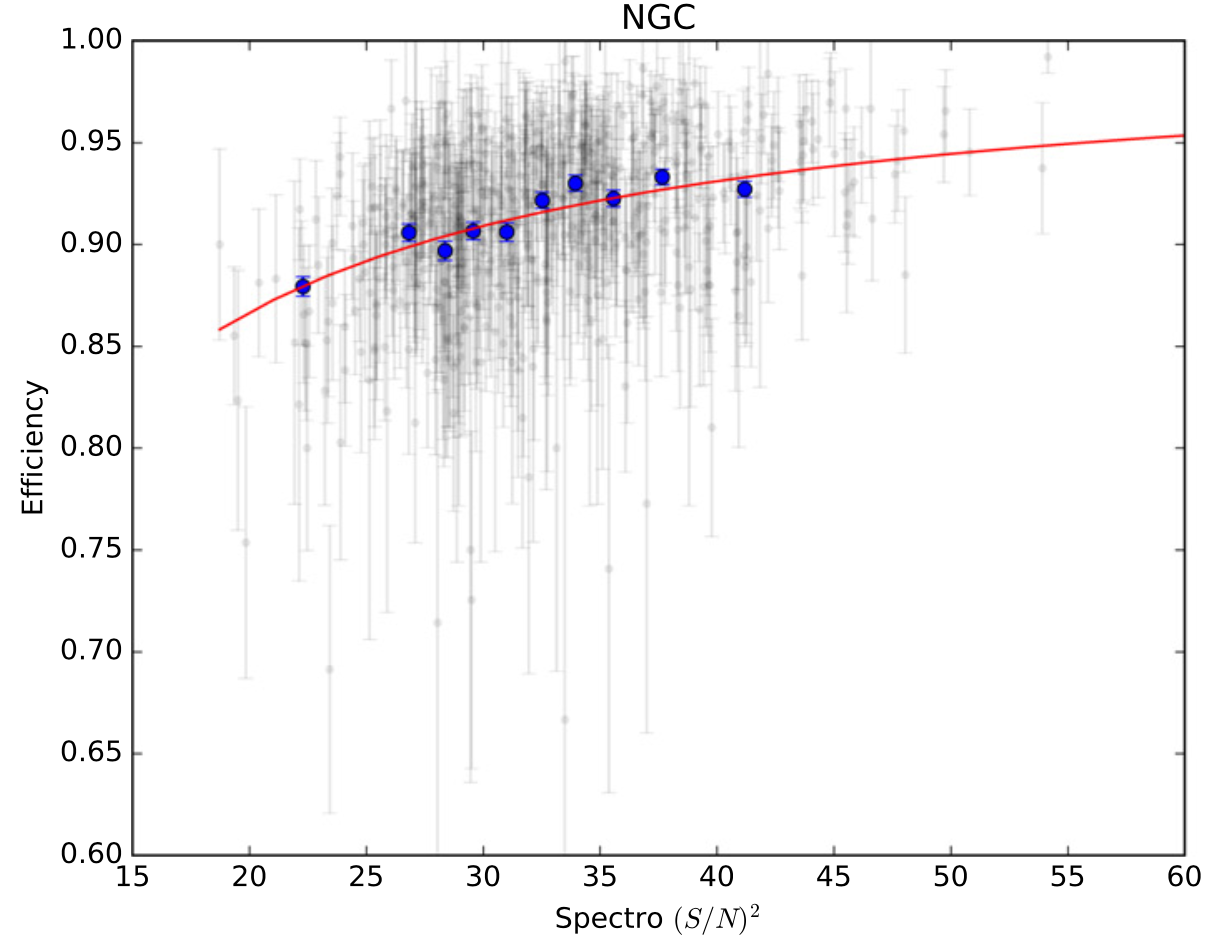
\includegraphics[width=0.49\textwidth]{fig/galaxies/eboss_z_failures_sn.png}
    \caption{ 
        Average redshift efficiency as a function of physical position of the optical 
        fiber in the focal plane (left panel) and as a function of the observation
        signal-to-noise squared (right panel).  
        The left panel shows how redshift-failures imprint a pattern on the sky 
        and therfore must be corrected. The right panel shows the underlying reason 
        for the failures. The model (red line) is used to compute correction weights.
    Figures extracted from \cite{bautistaSDSSIVExtendedBaryon2018}.} 
    \label{fig:eboss_zfailures}
\end{figure}

Once all galaxies have their correction weights (fibre collision, photometric and 
redshift-failure) and the randoms are corrected by fibre completeness, 
the radial selection function. The idea is to assign redshifts to randoms 
such that they follow the same redshift distribution as the galaxies. 
The redshift distribution is often quantified by the comoving galaxy (weighted)
number density $\bar{n}(z)$. 
Figure~\ref{fig:eboss_z_distrib} shows the comoving density of eBOSS tracers 
as a function of redshift. 
For randoms to match this distribution, we randomly assign the actual galaxy 
redshifts to each random, with repetition. Another possibility is to 
fit some smooth function over the observed $\bar{n}(z)$ and draw random redshifts
from the resulting model. In any case, these methods will introduce the so called 
\emph{radial integral constraint}, i.e., the fact that the observed $\bar{n}(z)$ is 
not the true ensemble averaged function of the Universe, it is just one 
volume-limited realisation of it. The impact on clustering of the radial integral 
constraint is inversely proportional to the area of the footprint
(\cite{demattiaIntegralConstraintsSpectroscopic2019}) and it is significant 
for surveys such as the eBOSS ELG (see Figure~\ref{fig:eboss_footprint} and 
\cite{tamoneCompletedSDSSIVExtended2020, demattiaCompletedSDSSIVExtended2021}). 


\begin{figure}
    \centering 
    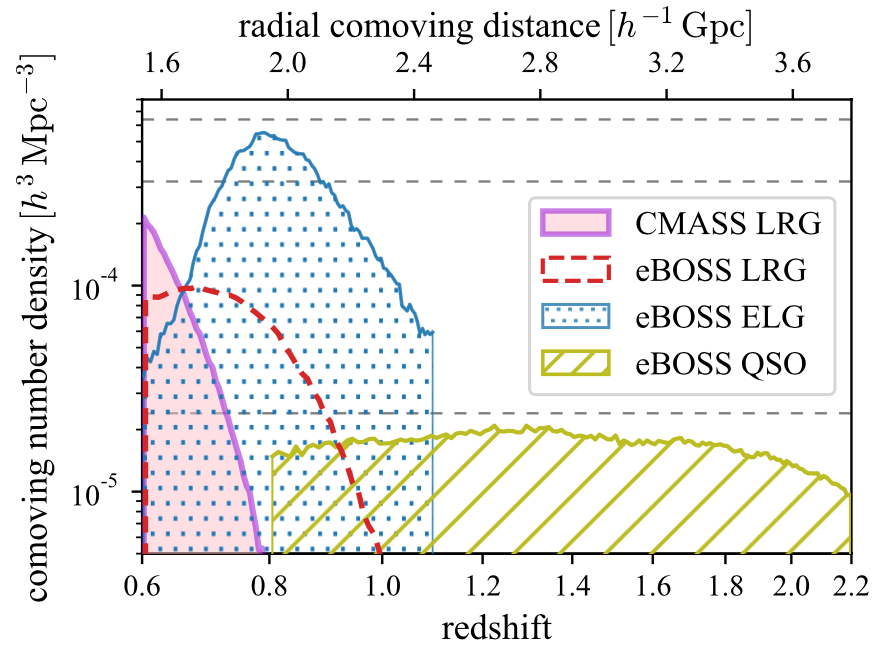
\includegraphics[width=0.6\textwidth]{fig/galaxies/eboss_z_distribution.png}
    \caption{ The weighted comoving number densities $\bar{n}(z)$ of eBOSS DR16 tracers
    and BOSS DR12 CMASS LRGs, with all the photometric and spectroscopic
    systematic weights included. 
    The comoving distances and volumes are computed assuming a flat-$\Lambda$CDM 
    cosmology with $\Omega_m = 0.31$. 
    %The three horizontal dashed lines show the number densities of the cubic LRG, ELG, and QSO    
    %EZmockcatalogues,i.e. $3.2 \times 10^{-4}$, $6.4 \times 10^{-4}$, and $2.4 \times 10^{-5} h^3 \text{Mpc}^{-3}$, respectively.
    Figure extracted from \cite{zhaoCompletedSDSSIVExtended2021}.} 
    \label{fig:eboss_z_distrib}
\end{figure}

The final step of the catalogue consists in adding an additional set of weights 
to galaxies that optimise the signal-to-noise ratio of clustering measurements 
when the redshift distribution is not uniform. These weights were first introduced 
by \cite{feldmanPowerSpectrumAnalysisThreedimensional1994} and have been applied 
to all clustering analysis ever since. They are commonly referred to as 
\emph{FKP weights} and can be written for a galaxy $i$ as
\begin{equation}
    w_\text{i, FKP} = \frac{1}{1 + \bar{n}(z_i)P_0}
\end{equation}
where $P_0$ is a rough value of the power spectrum of the tracers at some 
particular scale of choice, usually BAO scales for large-scale clustering measurements.
For eBOSS analyses, we chose a scale of $k \sim 0.1 h\, \text{Mpc}^{-1}$ for which 
$P_0 = 10000 h^{-3}\text{Mpc}^{3}$ for LRGs, 
$P_0 = 4000 h^{-3}\text{Mpc}^{3}$ for ELGs and 
$P_0 = 6000 h^{-3} \text{Mpc}^{3}$ for QSOs. 

As summary, the random catalogue describes the angular and radial selection functions
of the galaxy survey. 
Each random has a weight $w_r = w_\text{comp} w_\text{FKP}$, where $w_\text{comp}$ accounts
the spectroscopic completeness of targets and $w_\text{FKP}$ are optimal weights for clustering. 
Each galaxy has a weight given by $w_g = w_\text{col} w_\text{photo} w_\text{fail} w_\text{FKP}$,
where $w_\text{col}$ accouns for fibre collisions, $w_\text{photo}$ corrects fluctuations caused 
by photometry and $w_\text{fail}$ corrects redshift failures. 
These weights are used computing correlation functions or power spectra (see~\ref{galaxies:clustering}).

\section{Reconstruction of linear density field} 
\label{galaxies:reconstruction}

Bulk motions of galaxies on scales of tens of Mpc impact their two-point statistics, 
acting as a smoothing of the clustering (\cite{eisensteinRobustnessAcousticScale2007}).  
These motions smooth/broaden the BAO peak, reducing the precision on our measurement of its position. 
In the past decades, several methods have been proposed to reconstruct
the linear density field and remove these bulk motions from a galaxy survey,
therefore sharpening the BAO peak.
These methods are referred to as \emph{reconstruction} methods. 
Reconstruction is now an essential part of standard BAO measurements from galaxy surveys,
since they improve significantly their precision. 

The simplest form of reconstruction is based on a theoretical relationship between 
the galaxy density field on large scales (our observable) and the displacement field connecting 
the observed field (Eulerian frame) to its past version (Lagrangian frame). 
Lagrangian perturbation theory (LPT) can predict these displacements 
(see \cite{bernardeauLargeScaleStructureUniverse2002} for a review). 
To first order, the relation between displacements and density is linear 
(\cite{zeldovichGravitationalInstabilityApproximate1970}) and works quite well in 
recovering the linear BAO peak 
(\cite{nusserTracingLargeScaleFluctuations1992, eisensteinImprovingCosmologicalDistance2007}).
The first order LPT reconstruction is often called \emph{Zeldovich reconstruction}. 
Extending to second order LPT does not improve BAO reconstruction significantly 
(\cite{seoHighprecisionPredictionsAcoustic2010}) but it helps on recovering the 
velocity field (\cite{kitauraEstimatingCosmicVelocity2012}).
Zeldovich reconstruction has been used in all BAO measurements from SDSS (BOSS and eBOSS).
I implemented a python version\footnote{\url{https://github.com/julianbautista/eboss_clustering/}} of 
the Zeldovich reconstruction that uses Fast Fourier Transforms while accounting for the 
large angle effects 
(\cite{burdenEfficientReconstructionLinear2014, burdenReconstructionFourierSpace2015}). 
Alternatively, displacements can be computed 
in configuration space using finite difference approximations (\cite{padmanabhanCentDistance352012})
though these are slower and less precise than iterative FFTs. 

There are other backward reconstruction techniques such as those based on the least action principle (LAP).
First proposed by \cite{peeblesTracingGalaxyOrbits1989}, it was extended to cosmological applications 
by \cite{nusserLeastActionPrinciple2000, sarpaBAOReconstructionSwift2019}. 
\cite{sarpaExtendedFastAction2021} applied it for the BAO measurement of the BOSS DR12 galaxy sample. 

Reconstruction is essential to improve the precision on BAO measurements. However, 
due to imperfections in recovering the true initial conditions, 
reconstruction has not yet been used in attempts to derive cosmological 
constraints from the full-shape of the reconstructed two-point statistics.
Therefore, analysis of redshift-space distortions are based on the non reconstructed 
clustering (see section~\ref{galaxies:rsd}).  

\section{Mock catalogues}
\label{galaxies:mocks}

An important limitation in cosmology is that we only have a single realisation of our Universe. 
Therefore simulations are an essential tool to overcome this limitation. 

We can recognise two types of simulations mainly used in cosmology. First, 
n-body simulations (eventually including gas) solve numerically for the formation of structures
and are computationally expensive. They focus on the fully non-linear aspects and require a 
higher resolution setting, preventing them to simulate very large volumes or producing numerous 
realisations. N-body simulations are still the baseline for tests of perturbation theory models. 
The second type of simulations are the so-called \emph{mock catalogues} or simply \emph{mocks}. 
They are lower resolution and do not fully describe the non-linear clustering but they are 
faster to produce both in large volumes and in large number of realisations.
Their are key for the understanding of biases in best-fitted quantities and on their uncertainties. 
Given the large number of realisations, mocks have been used to estimate covariance matrices of 
clustering. Also, mocks allow us to study statistically the impact of observational systematic effects on our 
measurements. The last cosmological measurements from galaxy surveys have all an associated set of 
n-body simulations and a set of mock catalogues. I will describe the example I was involved in, 
the case of \textsc{EZmocks} produced for the eBOSS DR16 clustering measurements. 

A set of 1000 \textsc{EZmock} realisations was used in eBOSS DR16 clustering measurements 
for LRGs, ELGs and QSOs. They are fully described in \cite{zhaoCompletedSDSSIVExtended2021}. 
These mocks employ an effective Zeldovich approximation to evolve 
the density field in longer time steps (\cite{chuangEZmocksExtendingZel2015}). 
By construction, these mocks match the large-scale clustering 
of the target data sample, both 2 and 3-point statistics. 
They have some extra free parameters to simulate a biased galaxy sample. 
The eBOSS \textsc{EZmocks} also include light-cone effects produced by interpolating boxes
at different redshifts. 

The last step in the production of \textsc{EZmocks} was the addition of systematic effects. 
I was responsible of implementing all known observational effects from the data. 
A simple script\footnote{\url{https://github.com/julianbautista/eboss_clustering/blob/master/bin/ezmocks_add_systematics.py}}
gathers the information from the real catalogues and simulates fibre collisions, spurious 
fluctuations caused by photometry and spectroscopy (redshift failures). 
These contaminated mocks are then corrected using the same algorithms as for the real data, 
as described in section~\ref{galaxies:catalogue}. The clustering before and after adding 
those effects is extensively compared to real data (\cite{zhaoCompletedSDSSIVExtended2021}) 
and the agreement is found to be excellent on the scales of interest for BAO and RSD measurements. 



\section{From catalogues to clustering estimates}
\label{galaxies:clustering}

Correlation function estimation ... 
\begin{equation}
 \xi(r, \mu) = \frac{DD - 2DR}{RR} + 1 
 \label{eq:landy-szalay}
\end{equation}

Power spectrum estimation ... 
\begin{equation}
 P_\ell(k) = 
\end{equation}

Covariance matrix ...  

\begin{figure}
    \centering
    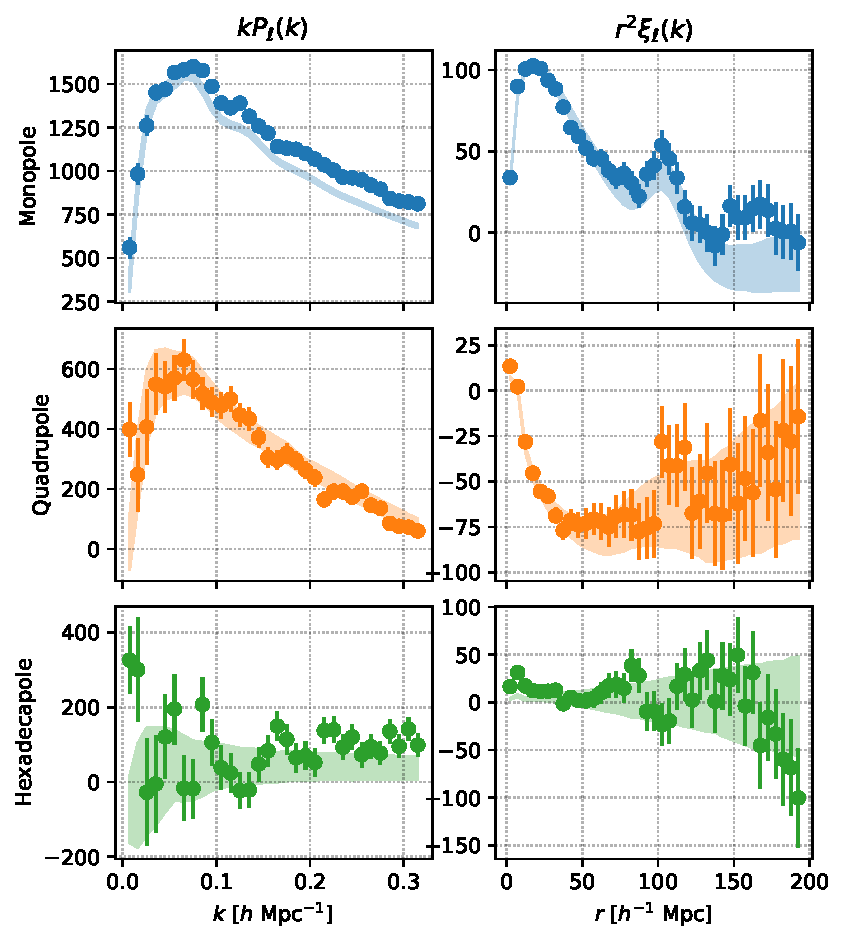
\includegraphics[width=0.8\textwidth]{fig/galaxies/DR16LRG_data_ezmock_prerecon.pdf}
    \caption{asd}
    \label{fig:LRG_data_ezmock_correlations_prerec}
\end{figure}

\begin{figure}
    \centering
    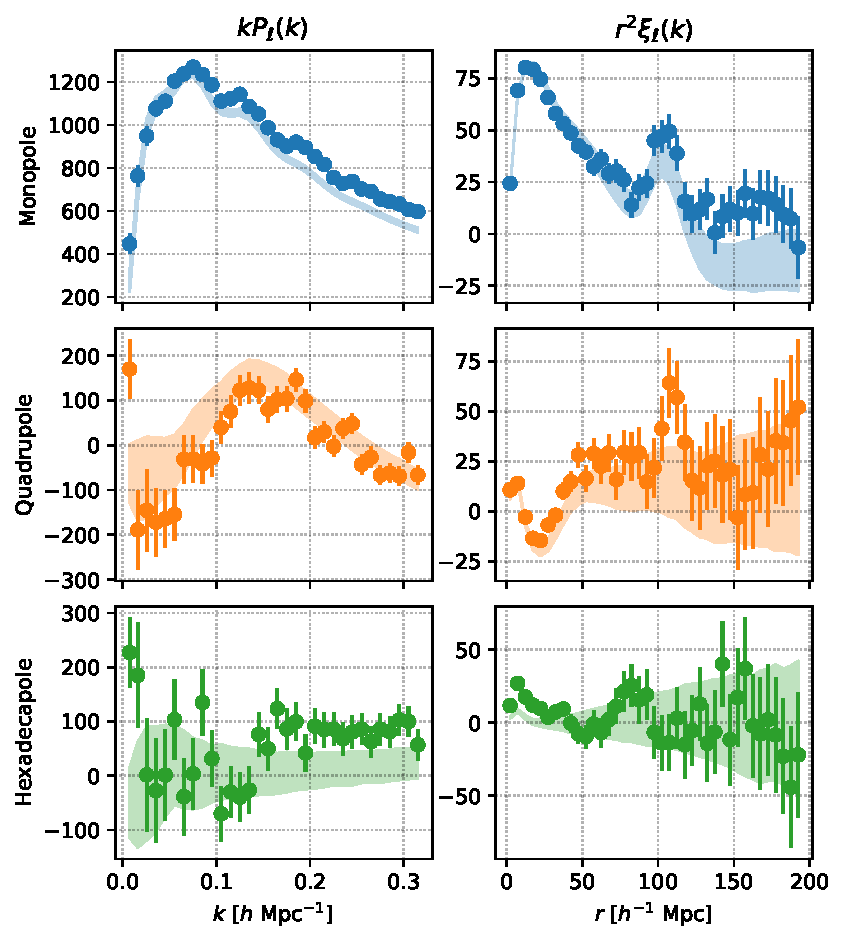
\includegraphics[width=0.8\textwidth]{fig/galaxies/DR16LRG_data_ezmock_postrecon.pdf}
    \caption{asd}
    \label{fig:LRG_data_ezmock_correlations_postrec}
\end{figure}


\section{Baryon acoustic oscillations}
\label{galaxies:bao}

Model 

Constraints with DR16 

\section{Redshift-space distortions}
\label{galaxies:rsd}

Model 

Constraints with DR16 

\section{Joint clustering analysis in Fourier and Configuration space}
\label{galaxies:joint}




\section{Cross-correlation with radio surveys}
\label{galaxies:radio}

\cite{wolzHIConstraintsCrosscorrelation2021}